\chapter{Image~Annotation}
\label{chap:annotation} 

This chapter describes the design, implementation of a human in the loop object detection system and details it's use annotating real datasets.

\section{Introduction}

\section {User interface}

The user interface of the system resembles a diagram editor, where shapes (boxes, circles, polygons) can be drawn over an image and manipulated in the usual ways. Shapes can be moved by selecting and dragging, resized by scrolling the mouse wheel or by moving control points. 


\subsection {Auto annotation}

At the core of the user interface is providing immediate feedback on images viewed by the user.


\subsection{Active learning}


\subsection {Confidence thresholding}

Choosing the confidence threshold is an important parameter for inference using an object detector. The consequence of an incorrect detection threshold is extra work for the annotator, either having to delete too many false positives or be left with too many boxes to draw. Many times, especially with difficult image detection problems an weak detector will produce many detections (some true positives, some false positives). The weak detector will not be able to separate these detections by confidence value. Using human verification there exist some obvious strategies to separate the true positives from the false positives, while still not missing too many objects altogether. 

\begin{itemize}
    \item Set a low detection threshold and have the user delete false positives
    \item Set a low detection threshold and have the user select true positives
    \item Set a high detection threshold and have the user draw boxes around missed detections
\end{itemize}

Each of these strategies has a valid place. If detections are so noisy and if the location predictions are very noisy (for example when the detector is very weak, such as near the start of the process) - having the user draw boxes is often the only option. Some of these strategies are amongst used by \cite{Konyushkova2017} which attempts to solve this problem differently, by attempting to automatically determine the best interface for a given image.

Deleting false positives is often the best option if true positives outnumber the false positives, or if the false positives are easy to select (if they're grouped together, for example). Selecting true positives is often the best option if the false positives outnumber the true positives. 
There exists another strategy which has the best of both worlds. Two thresholds can be used, a high confidence threshold can be used for eliminating false positives (such that when using this threshold the number of false positives is low). Detections between the high and low confidence thresholds can be considered for selection as true positives (such that the number of true positives requiring selection is low).


\begin{figure*}[h]
\centering
\begin{subfigure}[t]{0.5\linewidth}
  \includegraphics[width=1.0\linewidth]{figures/annotation/scallop/review_mode.png}
  \caption{}
\end{subfigure}%
\begin{subfigure}[t]{0.5\linewidth}
  \includegraphics[width=1.0\linewidth]{figures/annotation/scallop/false_positive.png}
  \caption{}
\end{subfigure}%
\caption{Review mode used on two fresh images from the scallop dataset, (a) showing an ideal case (b) showing an image with a high confidence false positive among low confidence detections}
\label {fig:confidence}
\end{figure*}



I provide a key which toggles between showing the detections in the mid range between the two thresholds, when the key is held a click is used to confirm a detection as a true positive. I term this toggle ``review mode''.  An example showing the mechanic of this can be seen in figure \ref{fig:scallop_review}. In one image the ideal situation is shown where three scallops are detected in the background (with low confidence), where otherwise they might have been ignored. In the other, a less useful case where the low confidence detections are false positives, and one of the high confidence detections is also a false positive, despite this the user saves time by ignoring the other low confidence detections.

The other advantage of this strategy are that it can bring the annotators attention to areas of the image which may have gone unnoticed. I have noticed in particular with the underwater scallop images that the detector usually did a good job at bringing attention to the more uncertain scallop instances. It also provides useful feedback to the annotator of the progress of the current object detector. 




\begin{figure}[h]
\centering
% \begin{subfigure}[b]
% %   \includegraphics[width=1.0\linewidth]{figures/annotation/confidence_training.pdf}
%   \caption{}
% \end{subfigure}

% \begin{subfigure}[b]
% %   \includegraphics[width=1.0\linewidth]{figures/annotation/confidence_validation.pdf}
%   \caption{}
% \end{subfigure}

\caption{ The evolution of confidence levels as training progresses, in (a) training and in (b) validation }
\label {fig:confidence}
\end{figure}

During training it can be seen that the confidence levels provided by the object detector vary with regard to training time. This can be seen in figure \ref{fig:confidence}, comparing the distribution of confidences between training and validation. This is a known property of neural network classifiers \cite{Guo2017}.

In future I would like to investigate calibration of thresholds using validation. This can be done by continually adjusting thresholds to match a certain ratio of false positives to false negatives (the desired ratio to be set by the user), alternatively prediction confidence itself can be calibrated to attempt to provide more consistent values. Confidence scores can be calibrated by scaling scaling outputs prior to applying softmax normalisation \cite{Guo2017}. For the purpose of object counting I use the former method to select thresholds. In order to provide the most unbiased estimate of counts the confidence is selected to give an equal ratio of false positives to negatives.


\subsection {Reviewing and verifying}

In crowd sourcing image annotation software, verification is required to ensure the consistency of the annotations. Verification prevents malicious or incompetent users to spoil the data and provides some assurance that the end result is of high quality. 



Reviewing a previously edited image and it's annotations is presented to the user in a very similar way to viewing a newly opened image. The main differences lie in how the global threshold affects the displayed annotations. 





\begin{figure}[h]
  \centering
  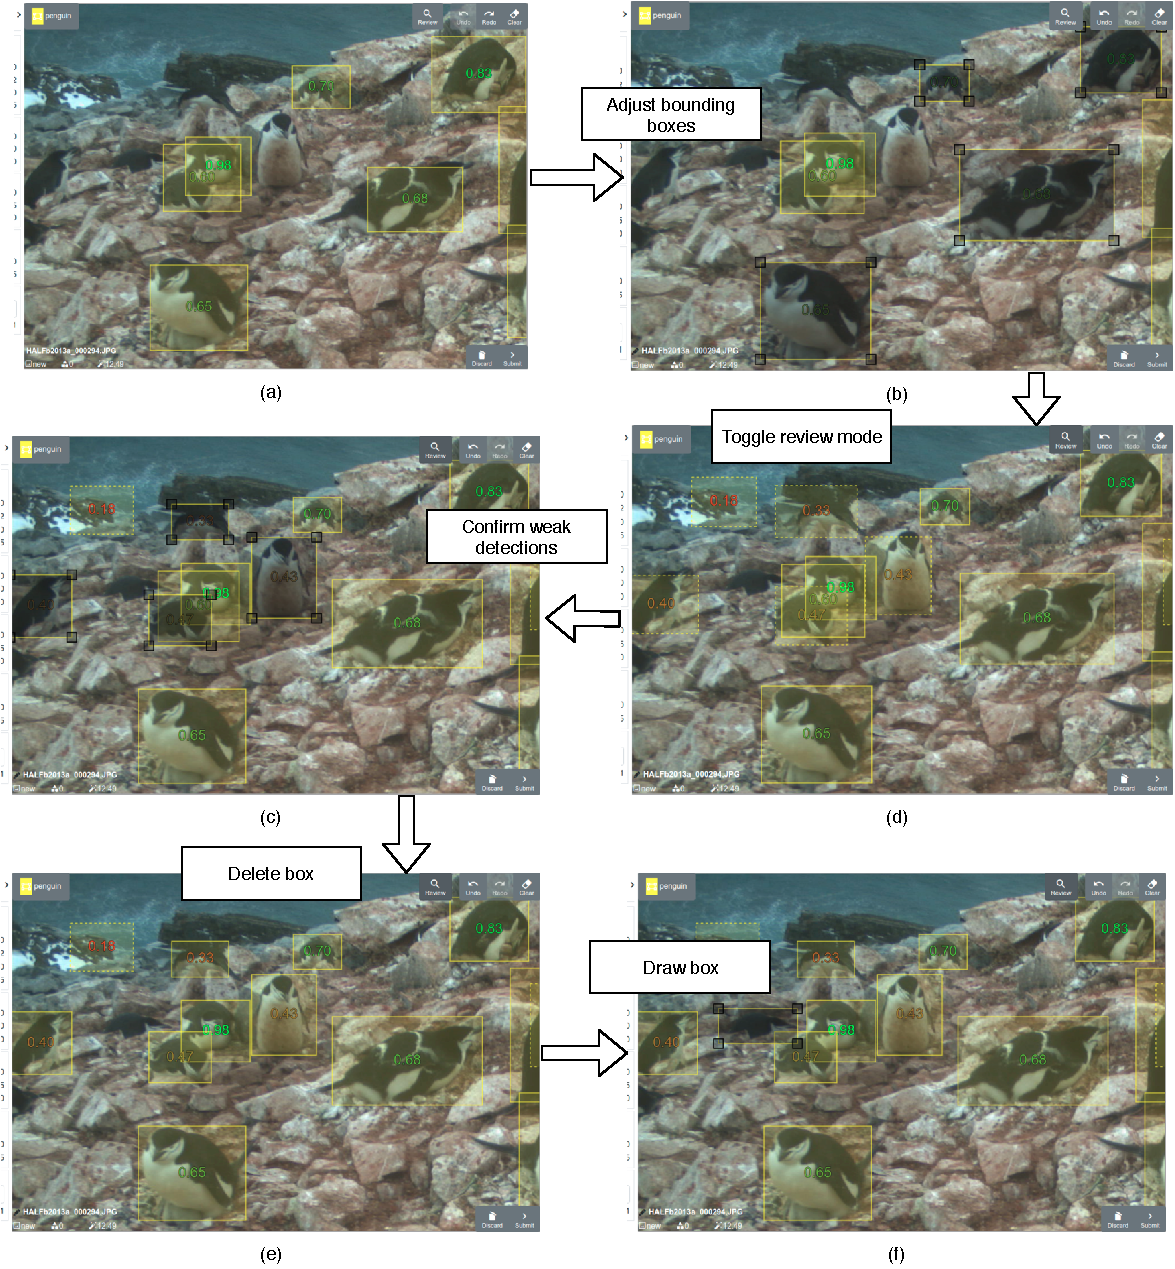
\includegraphics[width=1.0\linewidth]{figures/annotation/penguin_refine.pdf}
  \caption{Illustration of a human annotator refining a set of bounding box predictions }  
  \label{fig:penguin_refinement}
\end{figure}




\section {Implementation}

\subsection{Server and client}

\begin{figure}[h!]
  \centering
  \includegraphics[width=1.0\linewidth]{annotation/connectivity.pdf}
  \caption{Connectivity of the annotation system}  
  \label{fig:connectivity}
\end{figure}

The system can be broken down into three parts running separately but communicating. This can be seen in figure \ref{fig:connectivity}. There exists a server process which sits in the middle and acts as a conduit for communication, a store of data and a serialisation of state. The server sits in the middle and communicates with both trainers and clients.

The main reason for splitting server and trainer was initially for practical reasons, the client and server both written in \gls{GHC} Haskell, and deep learning frameworks written mainly in python. The server and client are written in Haskell, the former running naively, the later compiled to JavaScript using \gls{GHCJS}. 

Splitting server and trainer does also provide some advantages. It allows the server to act as a portal through which users can work on several datasets. One or many trainers can be shared concurrently or time shared without having to run new instances of the server. 

The current reality is more simple, a single trainer services the server and operates on a first come first served basis. One dataset at a time is trained, until a period of inactivity (no images submitted for $ n $ training epochs). A trainer still services clients working on inactive datasets by providing detection (best models for each dataset are kept in \gls{CPU} memory), but trains on only one dataset at a time. 

\begin{figure}[h!]
  \centering
  \includegraphics[width=1.0\linewidth]{annotation/data_flow.pdf}
  \caption{Data flow between services for the annotation system}  
  \label{fig:data_flow}
\end{figure}

An illustration of the data flow which occurs between different parties can be seen in figure \ref{fig:data_flow}. Large binary data is shared using \gls{HTTP}, for example model weights and images are distributed this way. Other data is communicated over websocket connections using \gls{JSON} text. Examples of this includes synchronising new annotations, and image statistics, which are continually updated to the client for the purpose of the example selection in active learning.

Image data is stored on the server and transmitted as required to trainer and client. Images are sent to client for viewing and inspection, and to the trainer for training and cached for more efficient loading. 

Models are stored on the server and requested by the trainer as required, for example when starting training on a dataset the trainer requests the previously stored model weights. The trainer also caches copies of weights (as required) of recently used models for the purposes of inference as required by the client for every image opened. Given the large size of data involved in transmitting large images, and also updating model weights, the trainer is suited to exist on the same local network as the server. 



\subsection {User interface}

I provide a web interface for the following reasons:

\begin{enumerate}
    \item No installation
\end{enumerate}
Any system with a web browser will be fine, software utilising complex computer vision and GPU programming libraries is often hard to package for easy installation. A web interface sidesteps these difficulties.
\begin{enumerate}[resume]
    \item Local GPU not required
\end{enumerate}
By running the trainer on another system anyone can use the system without requiring a local GPU. One of the problems with usability from my earlier work was that GPU intensive tasks running on the same computer ruin the responsiveness of a user interface. To my knowledge there is no good way to run a heavy \gls{GPU} intensive processing task at a low priority such that the user interface remains responsive.
\begin{enumerate}[resume]
    \item Enables collaborative annotation/crowd sourcing
\end{enumerate}
A web interface enables a straightforward extension to use for larger scale annotation with multiple users annotating the same dataset. An example can be seen in \label{fig:connectivity} showing two groups of users operating on the same datasets.


The trade-off for a web interface is in performance, it prevents doing computationally heavy calculation in the client, especially for loading and processing large images. For this work we face no such difficulty, though for example a super pixel based tool for mask annotation would be more challenging. With newer web technologies such as WebAssembly \cite{Haas2017} to run code at near native speeds in a browser, and WebGL shaders for GPU programming.











\section{Annotation studies}

\subsection {Penguins}
\subsection{Tree branch intersections}
\subsection{Scallop}


\section{Counting}

\subsection{Adelie Penguins}
\subsection{Waddell Seals}




\section {Reviewing mistakes}